%% bare_conf.tex
%% V1.3
%% 2007/01/11
%% by Michael Shell
%% See:
%% http://www.michaelshell.org/
%% for current contact information.
%%
%% This is a skeleton file demonstrating the use of IEEEtran.cls
%% (requires IEEEtran.cls version 1.7 or later) with an IEEE conference paper.
%%
%% Support sites:
%% http://www.michaelshell.org/tex/ieeetran/
%% http://www.ctan.org/tex-archive/macros/latex/contrib/IEEEtran/
%% and
%% http://www.ieee.org/

%%*************************************************************************
%% Legal Notice:
%% This code is offered as-is without any warranty either expressed or
%% implied; without even the implied warranty of MERCHANTABILITY or
%% FITNESS FOR A PARTICULAR PURPOSE! 
%% User assumes all risk.
%% In no event shall IEEE or any contributor to this code be liable for
%% any damages or losses, including, but not limited to, incidental,
%% consequential, or any other damages, resulting from the use or misuse
%% of any information contained here.
%%
%% All comments are the opinions of their respective authors and are not
%% necessarily endorsed by the IEEE.
%%
%% This work is distributed under the LaTeX Project Public License (LPPL)
%% ( http://www.latex-project.org/ ) version 1.3, and may be freely used,
%% distributed and modified. A copy of the LPPL, version 1.3, is included
%% in the base LaTeX documentation of all distributions of LaTeX released
%% 2003/12/01 or later.
%% Retain all contribution notices and credits.
%% ** Modified files should be clearly indicated as such, including  **
%% ** renaming them and changing author support contact information. **
%%
%% File list of work: IEEEtran.cls, IEEEtran_HOWTO.pdf, bare_adv.tex,
%%                    bare_conf.tex, bare_jrnl.tex, bare_jrnl_compsoc.tex
%%*************************************************************************

% *** Authors should verify (and, if needed, correct) their LaTeX system  ***
% *** with the testflow diagnostic prior to trusting their LaTeX platform ***
% *** with production work. IEEE's font choices can trigger bugs that do  ***
% *** not appear when using other class files.                            ***
% The testflow support page is at:
% http://www.michaelshell.org/tex/testflow/



% Note that the a4paper option is mainly intended so that authors in
% countries using A4 can easily print to A4 and see how their papers will
% look in print - the typesetting of the document will not typically be
% affected with changes in paper size (but the bottom and side margins will).
% Use the testflow package mentioned above to verify correct handling of
% both paper sizes by the user's LaTeX system.
%
% Also note that the "draftcls" or "draftclsnofoot", not "draft", option
% should be used if it is desired that the figures are to be displayed in
% draft mode.
%
\documentclass[conference]{IEEEtran}
% Add the compsoc option for Computer Society conferences.
%
% If IEEEtran.cls has not been installed into the LaTeX system files,
% manually specify the path to it like:
% \documentclass[conference]{../sty/IEEEtran}





% Some very useful LaTeX packages include:
% (uncomment the ones you want to load)


% *** MISC UTILITY PACKAGES ***
%
%\usepackage{ifpdf}
% Heiko Oberdiek's ifpdf.sty is very useful if you need conditional
% compilation based on whether the output is pdf or dvi.
% usage:
% \ifpdf
%   % pdf code
% \else
%   % dvi code
% \fi
% The latest version of ifpdf.sty can be obtained from:
% http://www.ctan.org/tex-archive/macros/latex/contrib/oberdiek/
% Also, note that IEEEtran.cls V1.7 and later provides a builtin
% \ifCLASSINFOpdf conditional that works the same way.
% When switching from latex to pdflatex and vice-versa, the compiler may
% have to be run twice to clear warning/error messages.






% *** CITATION PACKAGES ***
%
%\usepackage{cite}
% cite.sty was written by Donald Arseneau
% V1.6 and later of IEEEtran pre-defines the format of the cite.sty package
% \cite{} output to follow that of IEEE. Loading the cite package will
% result in citation numbers being automatically sorted and properly
% "compressed/ranged". e.g., [1], [9], [2], [7], [5], [6] without using
% cite.sty will become [1], [2], [5]--[7], [9] using cite.sty. cite.sty's
% \cite will automatically add leading space, if needed. Use cite.sty's
% noadjust option (cite.sty V3.8 and later) if you want to turn this off.
% cite.sty is already installed on most LaTeX systems. Be sure and use
% version 4.0 (2003-05-27) and later if using hyperref.sty. cite.sty does
% not currently provide for hyperlinked citations.
% The latest version can be obtained at:
% http://www.ctan.org/tex-archive/macros/latex/contrib/cite/
% The documentation is contained in the cite.sty file itself.






% *** GRAPHICS RELATED PACKAGES ***
%
\ifCLASSINFOpdf
  % \usepackage[pdftex]{graphicx}
  % declare the path(s) where your graphic files are
  % \graphicspath{{../pdf/}{../jpeg/}}
  % and their extensions so you won't have to specify these with
  % every instance of \includegraphics
  % \DeclareGraphicsExtensions{.pdf,.jpeg,.png}
\else
  % or other class option (dvipsone, dvipdf, if not using dvips). graphicx
  % will default to the driver specified in the system graphics.cfg if no
  % driver is specified.
  % \usepackage[dvips]{graphicx}
  % declare the path(s) where your graphic files are
  % \graphicspath{{../eps/}}
  % and their extensions so you won't have to specify these with
  % every instance of \includegraphics
  % \DeclareGraphicsExtensions{.eps}
\fi
% graphicx was written by David Carlisle and Sebastian Rahtz. It is
% required if you want graphics, photos, etc. graphicx.sty is already
% installed on most LaTeX systems. The latest version and documentation can
% be obtained at: 
% http://www.ctan.org/tex-archive/macros/latex/required/graphics/
% Another good source of documentation is "Using Imported Graphics in
% LaTeX2e" by Keith Reckdahl which can be found as epslatex.ps or
% epslatex.pdf at: http://www.ctan.org/tex-archive/info/
%
% latex, and pdflatex in dvi mode, support graphics in encapsulated
% postscript (.eps) format. pdflatex in pdf mode supports graphics
% in .pdf, .jpeg, .png and .mps (metapost) formats. Users should ensure
% that all non-photo figures use a vector format (.eps, .pdf, .mps) and
% not a bitmapped formats (.jpeg, .png). IEEE frowns on bitmapped formats
% which can result in "jaggedy"/blurry rendering of lines and letters as
% well as large increases in file sizes.
%
% You can find documentation about the pdfTeX application at:
% http://www.tug.org/applications/pdftex





% *** MATH PACKAGES ***
%
\usepackage[cmex10]{amsmath}
% A popular package from the American Mathematical Society that provides
% many useful and powerful commands for dealing with mathematics. If using
% it, be sure to load this package with the cmex10 option to ensure that
% only type 1 fonts will utilized at all point sizes. Without this option,
% it is possible that some math symbols, particularly those within
% footnotes, will be rendered in bitmap form which will result in a
% document that can not be IEEE Xplore compliant!
%
% Also, note that the amsmath package sets \interdisplaylinepenalty to 10000
% thus preventing page breaks from occurring within multiline equations. Use:
\interdisplaylinepenalty=2500
% after loading amsmath to restore such page breaks as IEEEtran.cls normally
% does. amsmath.sty is already installed on most LaTeX systems. The latest
% version and documentation can be obtained at:
% http://www.ctan.org/tex-archive/macros/latex/required/amslatex/math/





% *** SPECIALIZED LIST PACKAGES ***
%
%\usepackage{algorithmic}
% algorithmic.sty was written by Peter Williams and Rogerio Brito.
% This package provides an algorithmic environment fo describing algorithms.
% You can use the algorithmic environment in-text or within a figure
% environment to provide for a floating algorithm. Do NOT use the algorithm
% floating environment provided by algorithm.sty (by the same authors) or
% algorithm2e.sty (by Christophe Fiorio) as IEEE does not use dedicated
% algorithm float types and packages that provide these will not provide
% correct IEEE style captions. The latest version and documentation of
% algorithmic.sty can be obtained at:
% http://www.ctan.org/tex-archive/macros/latex/contrib/algorithms/
% There is also a support site at:
% http://algorithms.berlios.de/index.html
% Also of interest may be the (relatively newer and more customizable)
% algorithmicx.sty package by Szasz Janos:
% http://www.ctan.org/tex-archive/macros/latex/contrib/algorithmicx/




% *** ALIGNMENT PACKAGES ***
%
%\usepackage{array}
% Frank Mittelbach's and David Carlisle's array.sty patches and improves
% the standard LaTeX2e array and tabular environments to provide better
% appearance and additional user controls. As the default LaTeX2e table
% generation code is lacking to the point of almost being broken with
% respect to the quality of the end results, all users are strongly
% advised to use an enhanced (at the very least that provided by array.sty)
% set of table tools. array.sty is already installed on most systems. The
% latest version and documentation can be obtained at:
% http://www.ctan.org/tex-archive/macros/latex/required/tools/


%\usepackage{mdwmath}
%\usepackage{mdwtab}
% Also highly recommended is Mark Wooding's extremely powerful MDW tools,
% especially mdwmath.sty and mdwtab.sty which are used to format equations
% and tables, respectively. The MDWtools set is already installed on most
% LaTeX systems. The lastest version and documentation is available at:
% http://www.ctan.org/tex-archive/macros/latex/contrib/mdwtools/


% IEEEtran contains the IEEEeqnarray family of commands that can be used to
% generate multiline equations as well as matrices, tables, etc., of high
% quality.


%\usepackage{eqparbox}
% Also of notable interest is Scott Pakin's eqparbox package for creating
% (automatically sized) equal width boxes - aka "natural width parboxes".
% Available at:
% http://www.ctan.org/tex-archive/macros/latex/contrib/eqparbox/





% *** SUBFIGURE PACKAGES ***
%\usepackage[tight,footnotesize]{subfigure}
% subfigure.sty was written by Steven Douglas Cochran. This package makes it
% easy to put subfigures in your figures. e.g., "Figure 1a and 1b". For IEEE
% work, it is a good idea to load it with the tight package option to reduce
% the amount of white space around the subfigures. subfigure.sty is already
% installed on most LaTeX systems. The latest version and documentation can
% be obtained at:
% http://www.ctan.org/tex-archive/obsolete/macros/latex/contrib/subfigure/
% subfigure.sty has been superceeded by subfig.sty.



%\usepackage[caption=false]{caption}
%\usepackage[font=footnotesize]{subfig}
% subfig.sty, also written by Steven Douglas Cochran, is the modern
% replacement for subfigure.sty. However, subfig.sty requires and
% automatically loads Axel Sommerfeldt's caption.sty which will override
% IEEEtran.cls handling of captions and this will result in nonIEEE style
% figure/table captions. To prevent this problem, be sure and preload
% caption.sty with its "caption=false" package option. This is will preserve
% IEEEtran.cls handing of captions. Version 1.3 (2005/06/28) and later 
% (recommended due to many improvements over 1.2) of subfig.sty supports
% the caption=false option directly:
\usepackage[caption=false,font=footnotesize]{subfig}
%
% The latest version and documentation can be obtained at:
% http://www.ctan.org/tex-archive/macros/latex/contrib/subfig/
% The latest version and documentation of caption.sty can be obtained at:
% http://www.ctan.org/tex-archive/macros/latex/contrib/caption/




% *** FLOAT PACKAGES ***
%
%\usepackage{fixltx2e}
% fixltx2e, the successor to the earlier fix2col.sty, was written by
% Frank Mittelbach and David Carlisle. This package corrects a few problems
% in the LaTeX2e kernel, the most notable of which is that in current
% LaTeX2e releases, the ordering of single and double column floats is not
% guaranteed to be preserved. Thus, an unpatched LaTeX2e can allow a
% single column figure to be placed prior to an earlier double column
% figure. The latest version and documentation can be found at:
% http://www.ctan.org/tex-archive/macros/latex/base/



%\usepackage{stfloats}
% stfloats.sty was written by Sigitas Tolusis. This package gives LaTeX2e
% the ability to do double column floats at the bottom of the page as well
% as the top. (e.g., "\begin{figure*}[!b]" is not normally possible in
% LaTeX2e). It also provides a command:
%\fnbelowfloat
% to enable the placement of footnotes below bottom floats (the standard
% LaTeX2e kernel puts them above bottom floats). This is an invasive package
% which rewrites many portions of the LaTeX2e float routines. It may not work
% with other packages that modify the LaTeX2e float routines. The latest
% version and documentation can be obtained at:
% http://www.ctan.org/tex-archive/macros/latex/contrib/sttools/
% Documentation is contained in the stfloats.sty comments as well as in the
% presfull.pdf file. Do not use the stfloats baselinefloat ability as IEEE
% does not allow \baselineskip to stretch. Authors submitting work to the
% IEEE should note that IEEE rarely uses double column equations and
% that authors should try to avoid such use. Do not be tempted to use the
% cuted.sty or midfloat.sty packages (also by Sigitas Tolusis) as IEEE does
% not format its papers in such ways.





% *** PDF, URL AND HYPERLINK PACKAGES ***
%
\usepackage{url}
% url.sty was written by Donald Arseneau. It provides better support for
% handling and breaking URLs. url.sty is already installed on most LaTeX
% systems. The latest version can be obtained at:
% http://www.ctan.org/tex-archive/macros/latex/contrib/misc/
% Read the url.sty source comments for usage information. Basically,
% \url{my_url_here}.





% *** Do not adjust lengths that control margins, column widths, etc. ***
% *** Do not use packages that alter fonts (such as pslatex).         ***
% There should be no need to do such things with IEEEtran.cls V1.6 and later.
% (Unless specifically asked to do so by the journal or conference you plan
% to submit to, of course. )

\usepackage[czech, english]{babel}
\usepackage[cp1250]{inputenc} % for win1250
\usepackage{graphicx}
\usepackage{cases}

% correct bad hyphenation here
\hyphenation{op-tical net-works semi-conduc-tor}


\begin{document}
\selectlanguage{english}
%
% paper title
% can use linebreaks \\ within to get better formatting as desired
\title{Road lighting design by means of genetic algorithm}


% author names and affiliations
% use a multiple column layout for up to three different
% affiliations
\selectlanguage{czech}

\author{
\IEEEauthorblockN{
Rudolf Bayer\IEEEauthorrefmark{1}, 
Michal Brejcha\IEEEauthorrefmark{2}, 
Jan Z�le��k\IEEEauthorrefmark{1}, 
Zuzana Pansk�\IEEEauthorrefmark{1} 
Marek B�lsk�\IEEEauthorrefmark{1}}

\IEEEauthorblockA{
\IEEEauthorrefmark{1}CTU in Prague, Faculty of Electrical Engineering, Department of Electrical Power Engineering\\
Praha 6, Technick� 2, 166 27\\
Email: bayerrud@fel.cvut.cz\\}

\IEEEauthorblockA{
\IEEEauthorrefmark{2}CTU in Prague, Faculty of Electrical Engineering, Department of Electrotechnology\\
Praha 6, Technick� 2, 166 27\\
Email: brejcmic@fel.cvut.cz}
}

\selectlanguage{english}
% conference papers do not typically use \thanks and this command
% is locked out in conference mode. If really needed, such as for
% the acknowledgment of grants, issue a \IEEEoverridecommandlockouts
% after \documentclass

% for over three affiliations, or if they all won't fit within the width
% of the page, use this alternative format:
% 
%\author{\IEEEauthorblockN{Michael Shell\IEEEauthorrefmark{1},
%Homer Simpson\IEEEauthorrefmark{2},
%James Kirk\IEEEauthorrefmark{3}, 
%Montgomery Scott\IEEEauthorrefmark{3} and
%Eldon Tyrell\IEEEauthorrefmark{4}}
%\IEEEauthorblockA{\IEEEauthorrefmark{1}School of Electrical and Computer Engineering\\
%Georgia Institute of Technology,
%Atlanta, Georgia 30332--0250\\ Email: see http://www.michaelshell.org/contact.html}
%\IEEEauthorblockA{\IEEEauthorrefmark{2}Twentieth Century Fox, Springfield, USA\\
%Email: homer@thesimpsons.com}
%\IEEEauthorblockA{\IEEEauthorrefmark{3}Starfleet Academy, San Francisco, California 96678-2391\\
%Telephone: (800) 555--1212, Fax: (888) 555--1212}
%\IEEEauthorblockA{\IEEEauthorrefmark{4}Tyrell Inc., 123 Replicant Street, Los Angeles, California 90210--4321}}




% use for special paper notices
%\IEEEspecialpapernotice{(Invited Paper)}




% make the title area
\maketitle


\begin{abstract}
%\boldmath
The abstract goes here.
\end{abstract}
% IEEEtran.cls defaults to using nonbold math in the Abstract.
% This preserves the distinction between vectors and scalars. However,
% if the conference you are submitting to favors bold math in the abstract,
% then you can use LaTeX's standard command \boldmath at the very start
% of the abstract to achieve this. Many IEEE journals/conferences frown on
% math in the abstract anyway.

% no keywords




% For peer review papers, you can put extra information on the cover
% page as needed:
% \ifCLASSOPTIONpeerreview
% \begin{center} \bfseries EDICS Category: 3-BBND \end{center}
% \fi
%
% For peerreview papers, this IEEEtran command inserts a page break and
% creates the second title. It will be ignored for other modes.
\IEEEpeerreviewmaketitle



\section{Introduction}
% no \IEEEPARstart
This demo file is intended to serve as a ``starter file''
for IEEE conference papers produced under \LaTeX\ using
IEEEtran.cls version 1.7 and later.
% You must have at least 2 lines in the paragraph with the drop letter
% (should never be an issue)
I wish you the best of success.

\hfill mds
 
\hfill January 11, 2007

\section{Road Lighting Design}
\label{sec:Road_Lighting_Design}
Lighting system designs of public roads in the Czech Republic have to meet among others the Czech Technical Standard \cite{CSN_EN_13201-2}. For this project a road for mainly cyclists but also for pedestrians has been chosen, that is according to \cite{CSN_EN_13201-1} lighting situation C1 and lighting class S4. Road lighting conforming to this class must meet in terms of \cite{CSN_EN_13201-2} the requirement of maintained average horizontal illuminance $\overline{E}_{M}\geq 5$ \textit{lx}, minimum maintained illuminance $E_{min,M}\geq 1$ \textit{lx} and uniformity so that the actual $\overline{E}_{M}$ must not exceed 1.5 times the minimal allowed $\overline{E}_{M}$ for the given lighting class, which is for class S4 $\overline{E}_{max,M} = 7.5$ \textit{lx}.

The maintenance factor $MF$ is another entry that has to be taken into account. This factor defines the depreciation of the design level, in this case the depreciation of illuminance $\overline{E}_{M}$ and $E_{min,M}$ over the course of operation of the road lighting. After choosing the luminaire Atos from Schr\'{e}der as the luminaire to be used throughout this project, the maintenance factor can be calculated from \cite{CSN_EN_13201-2_Z1}:
\begin{equation} \label{eq:MF}
MF = LLMF \cdot LSF \cdot LMF
\end{equation}
Where:
\begin{description}
	\item[$LLMF$] is the lamp lumen maintenance factor
	\item[$LSF$] is the lamp survival factor
	\item[$LMF$] is the luminaire factor
\end{description}

The Atos luminaire's are fitted with high pressure sodium lamps. For this project Osram NAV-T 70 W super 6Y and Osram NAV-T 50 W super 6Y have been chosen to operate for a period of 12000 hours before replacement. Looking up the product datasheet \cite{Osram} of both 70 W and 50 W Osram lamps, $LLMF_{70W}=0.89$, $LLMF_{50W}=0.86$, $LSF_{70W}=0.97$ and $LSF_{50W}=0.97$ can be found. The IP Code of the luminaire's optical system is IP66, meaning that for an environment of medium air pollution and cleaning intervals of 2 years $LMF=0.89$ can be found in table NA.1 of \cite{CSN_EN_13201-2_Z1}. According to equation~\ref{eq:MF} the final maintenance factors can be calculated as follows:

\begin{align}
&MF_{70W} = 0.89 \cdot 0.97 \cdot 0.89 = 0.785603\\
&MF_{50W} = 0.86 \cdot 0.97 \cdot 0.89 = 0.742438
\end{align}

Where:
\begin{description}
	\item[$MF_{70W}$] is the maintenance factor for the 70 Watt Osram sodium lamp
	\item[$MF_{50W}$] is the maintenance factor for the 50 Watt Osram sodium lamp
\end{description}

To obtain the initially required illuminances of $\overline{E}$ and $E_{min}$ at the beginning of the road lighting operation, maintenance factors have to be taken into account:
\begin{equation}
E = E_{M} \div MF
\end{equation}
Where:
\begin{description}
	\item[$E$] is the general illuminance value calculated or measured at the beginning of the operation cycle
	\item[$E_{M}$] is the maintained illuminance value assumed at the end of the operation cycle
	\item[$MF$] is the maintenance factor
\end{description}

Having calculated both maintenance factors, the initial illuminances can be specified:

\begin{align}
&\overline{E}_{70W} = \overline{E}_{M} \div MF_{70W} \doteq 6.36 \textit{ lx}\\
&\overline{E}_{max,70W} = \overline{E}_{max,M} \div MF_{70W} \doteq 9.55 \textit{ lx}\\
&\overline{E}_{min,70W} = \overline{E}_{min,M} \div MF_{70W} \doteq 1.27 \textit{ lx}\\
&\overline{E}_{50W} = \overline{E}_{M} \div MF_{50W} \doteq 6.73 \textit{ lx}\\
&\overline{E}_{max,50W} = \overline{E}_{max,M} \div MF_{50W} \doteq 10.10 \textit{ lx}\\
&\overline{E}_{min,50W} = \overline{E}_{min,M} \div MF_{50W} \doteq 1.34 \textit{ lx}
\end{align}

\section{Illuminance calculation}
Illuminance $E$ of a planar surface is the areal density of luminous flux incident on the surface \cite{Habel}:

\begin{equation}
E=\frac{d\Phi_{i}}{dA}
\end{equation}

Where:
\begin{description}
	\item[$d\Phi_{i}$] is the luminous flux incident on a surface
	\item[$dA$] is the surface area
\end{description}

Luminous intensity $I$ is the amount of luminous flux contained in a given solid angle. For a direction defined by angle $\gamma$ is luminous intensity of this angle defined as follows \cite{Habel}:

\begin{equation}
I_{\gamma}=\frac{d\Phi}{d\Omega}
\end{equation}

Where:
\begin{description}
	\item[$d\Phi$] is the amount of luminous flux contained in the solid angle $d\Omega$
	\item[$d\Omega$] is the solid angle with its axis pointing in direction~$\gamma$
\end{description}

As mentioned in section~\ref{sec:Road_Lighting_Design}, illuminances need to be calculated. Photometric properties of luminaires are defined in eulumdat files, containing luminous intensity distribution curves needed to obtain illuminances.

\begin{figure}[htb]
  \centering
  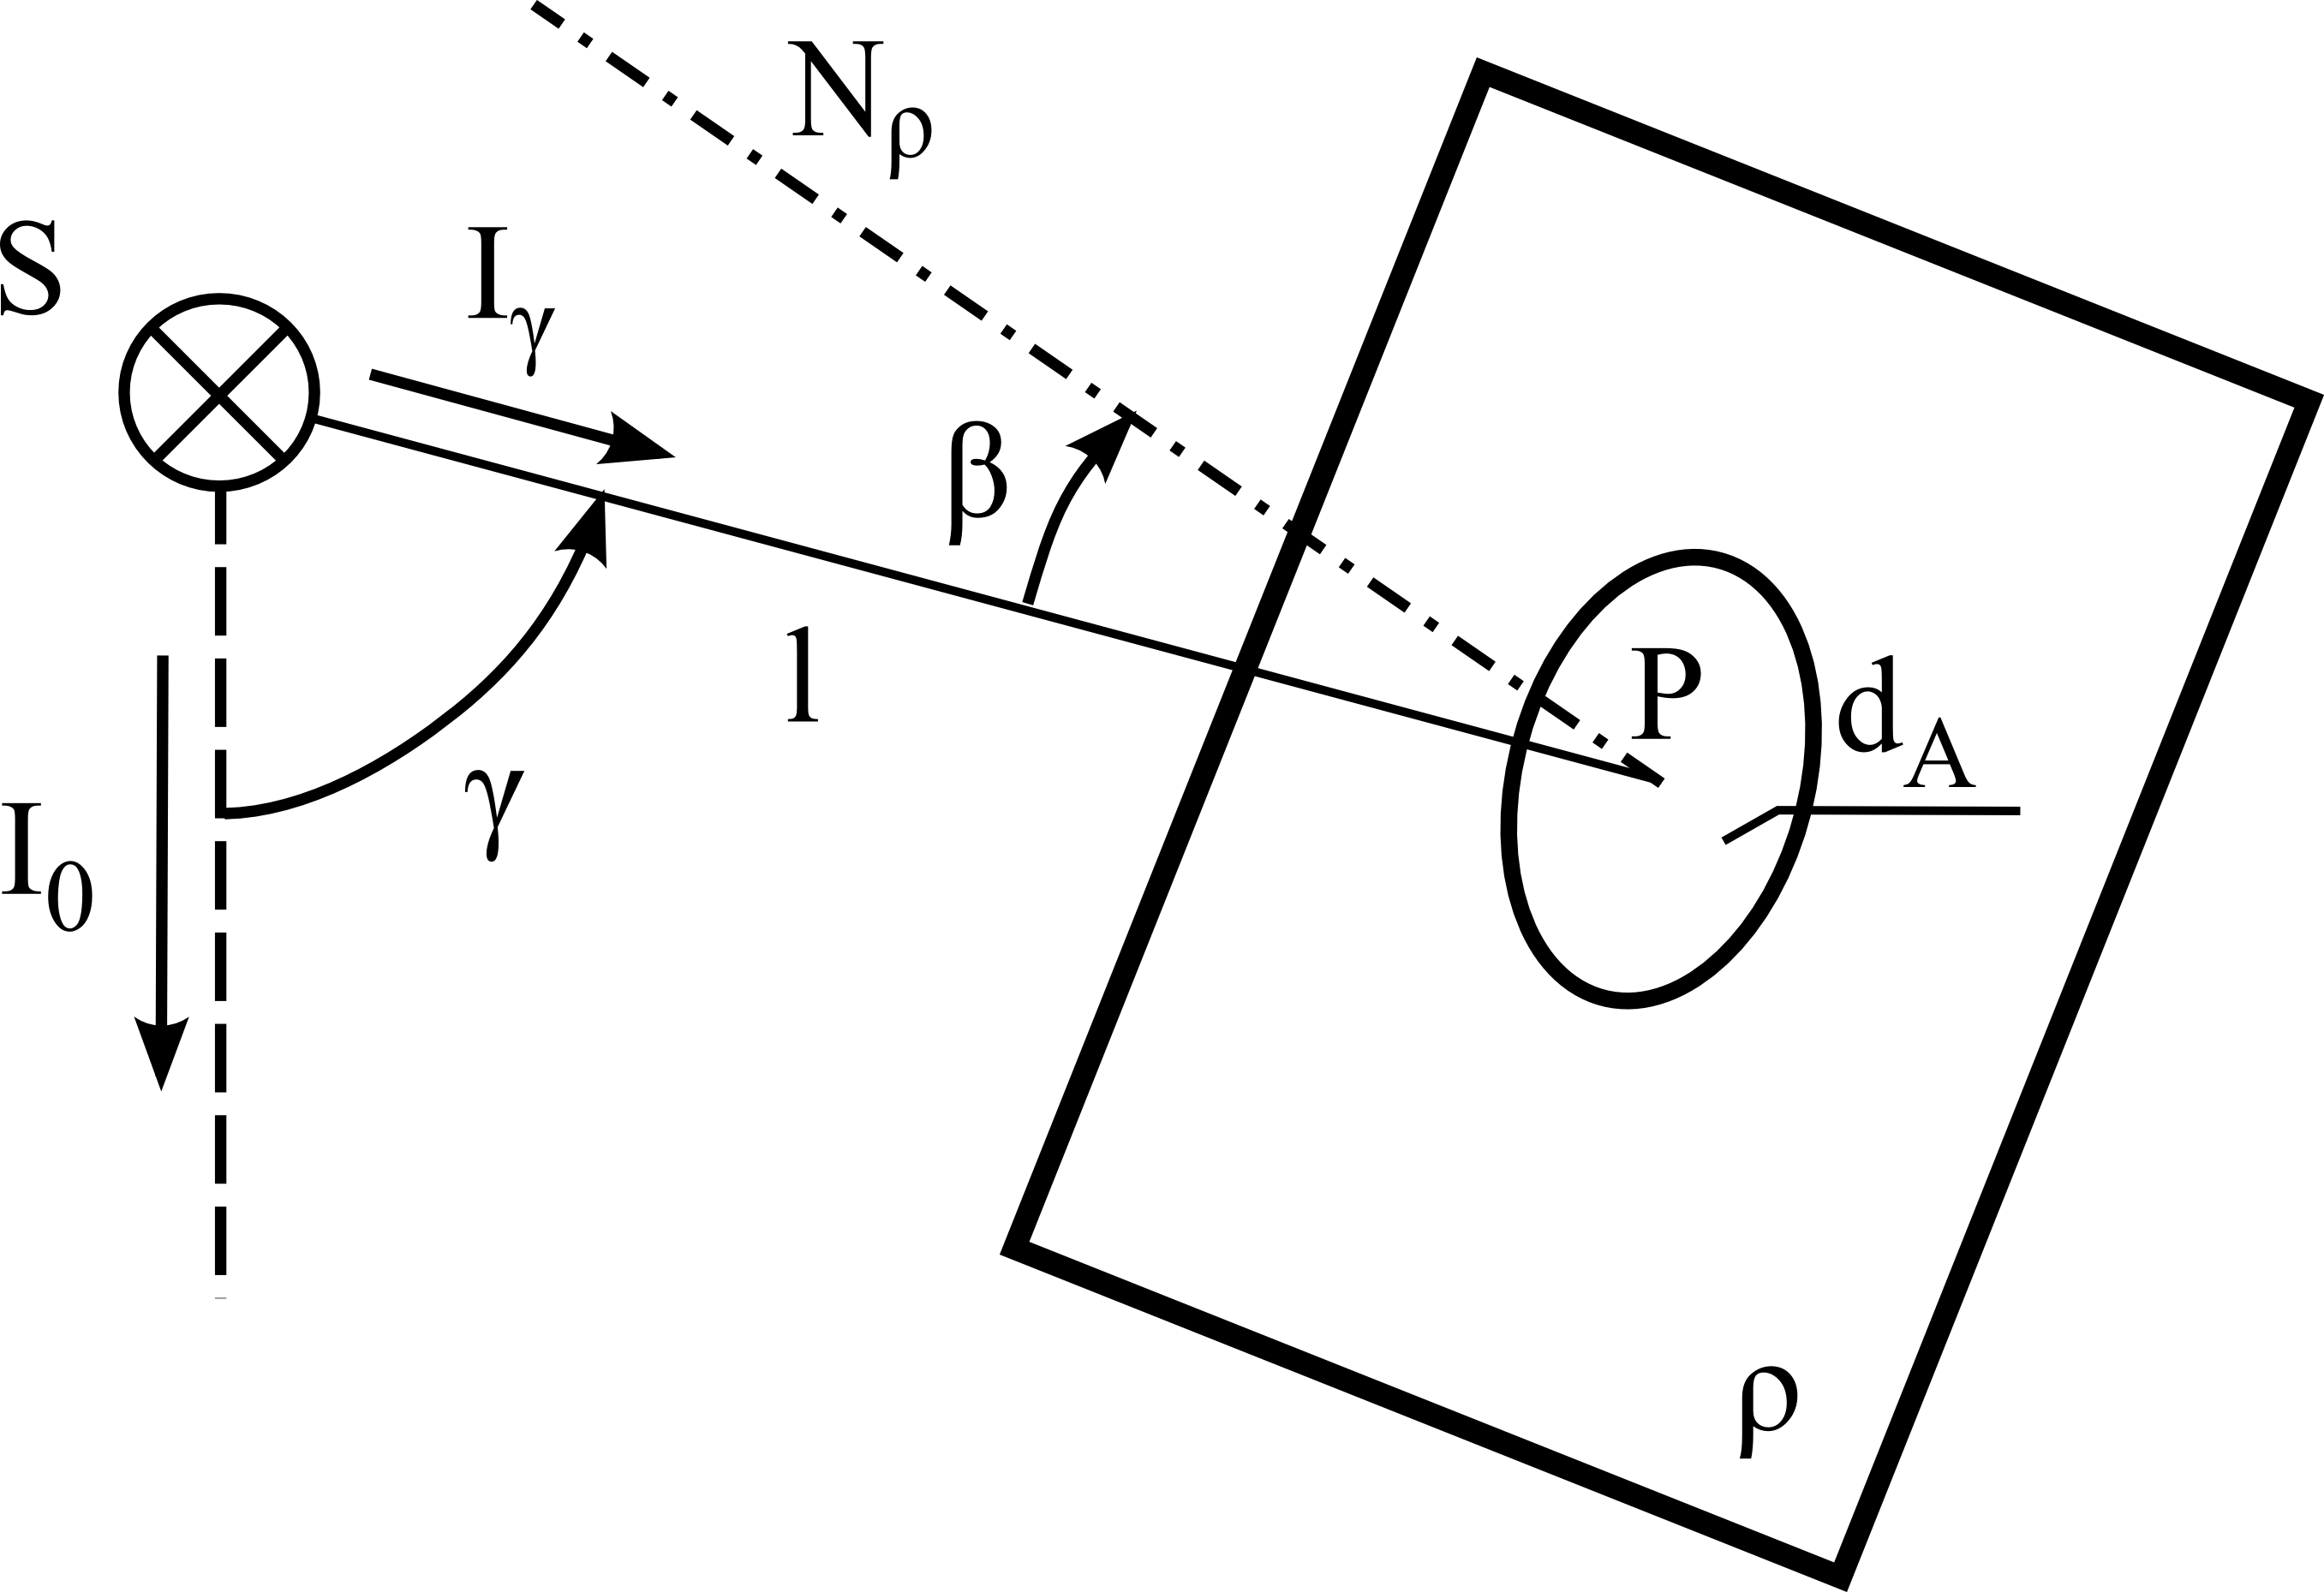
\includegraphics[width=0.8\columnwidth]{315_osvetlenost_bodovym_zdrojem}
  \caption{Facet $\rho$ illuminated with light source $S$}
  \label{fig:illuminance}
\end{figure}

According to~\cite{Habel} illuminance at point $P$ (as seen in figure~\ref{fig:illuminance}) illuminated by light source $S$ can be obtained by the following equation:

\begin{equation}
E_{P\rho}=\frac{I_{\gamma} \cdot cos \beta}{l^2}
\end{equation}

Where:
\begin{description}
	\item[$I_{\gamma}$] is the luminous intensity in the given direction $\gamma$
	\item[$\beta$] is the angle between the surface's normal $N_{\rho}$ and the $SP$ point join $l$
	\item[$l$] is the distance between the light source S and the point P of facet $dA$ of surface $\rho$
\end{description}


\section{Luminaire Parameters}
For the calculations one type of luminaire has been chosen. From a wide range of outdoor luminaire procuders and distributors at the Czech market the luminaire Atos of the Schr\'{e}der company has been chosen. Atos luminaires are nowadays widely used for public outdoor lighting and can be fitted with light sources from 50~W to 150~W, making it suitable for road lighting of lower categories, e.g. pedestrian zones, cycleways, emergency lanes etc.

The adjustment of luminous intensity distribution curves can be achieved by a displacement of the light source inside the luminaire. The luminaire Atos offers 12 positions of the light source inside the luminaire, therefore 12 different luminous intensity distribution curves can be obtained. 

\begin{figure}[htb]
  \centering
  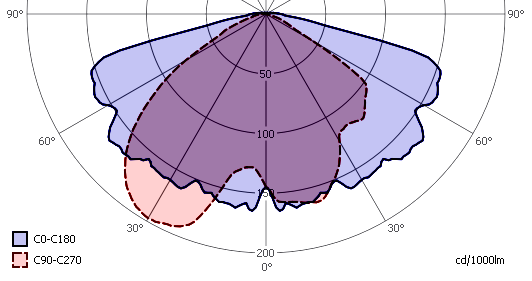
\includegraphics[width=\columnwidth]{70W_A1_v2}
  \caption{Luminous intensity distribution curves of ATOS/1627/SMOOTH POLYCARBONATE/SON-T 70/-17/100/10$^\circ$}
  \label{fig:lumIntDistr}
\end{figure}

\begin{figure}[htb]
  \centering
  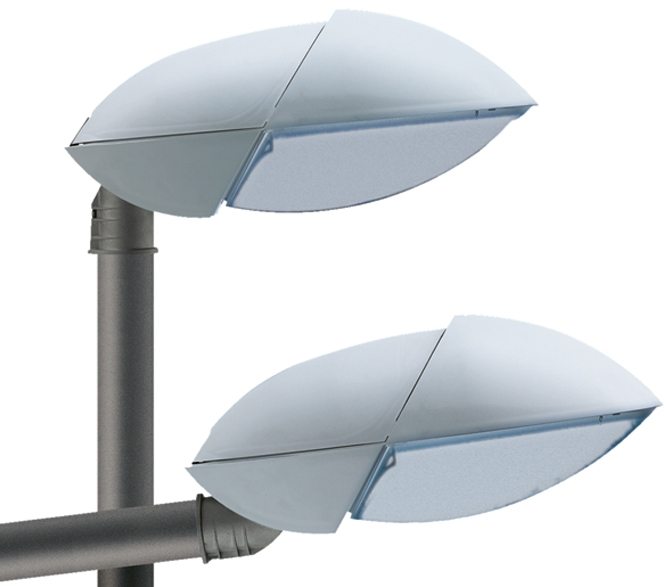
\includegraphics[width=0.7\columnwidth]{Atos}
  \caption{A photograph of the luminaire Atos}
  \label{fig:lumIntDistr}
\end{figure}

\section{Genetic Algorithm Introduction}
The genetic algorithms (GA) are the part of the evolutionary computing. Similar to the living organism are the solutions represented by their genotype, that represents the parameter coding and by phenotype, that represents behaviour, response and features of the solutions. The genotype is typically coded as a vector of parameters termed a chromosome, with elements being described as genes~\cite{Fogel2006}. Each solution is considered according to its phenotype and selected if the phenotype fits the constraints and conditions of an examined environment or task. The ability to survive and reproduce in specific environment is called fitness. The Selection must maintain or increase the fitness of solution sets that are called populations. Each set of solutions corresponds to one so called generation.

Each generation starts with selecting solutions with high fitness to form set of parent solutions for the next population. After that the process of crossovers and mutations creates new population. The crossover combines two chromosomes of parent solutions together. The one-point crossover was used in presented solutions. Parent chromosomes are randomly split at the same point and the parts that follow that point are exchanged. The mutation changes the chromosome directly. It can change the value of a selected gene for example. The paper deals with the implemented mutation in the next section. Both the crossovers and mutations are made only with certain probability. The probability of crossovers is typically high (more than 90~\%) in comparison to mutation, which must be low (under 10~\%). High probability of mutation makes the optimization difficult because of the high rate of change in chromosomes.

\section{Results Consideration}

\begin{table}[htb]
	\renewcommand{\arraystretch}{1.3}
	\caption{Results for one side lamp placement}
 	\label{tab:onesideLamps}
	\centering
  \begin{tabular}{ l | c | c | c | c | c | c }
    \hline
    \textbf{Type} & $D_X$ & $D_Y$ & $Z$ & $\alpha$ & $E_{avg}$ & $E_{min}$\\ 
    & (m) & (m) & (m) & ($^\circ$) & (lx) & (lx)\\ \hline
    ATOS 70W A1 & 40.2 & 1.15 & 6.71 & 0.18 & 7.62 & 1.34 \\ \hline
    ATOS 70W A2 & 40.2 & 0.02 & 6.04 & 13.46 & 7.71 & 1.25\\ \hline
    ATOS 70W A3 & 43.5 & 0.58 & 7.41 & 2.04 & 7.74 & 1.72\\ \hline
    ATOS 70W A4 & 48.4 & -0.16 & 7.30 & 3.07 & 7.65 & 1.54\\ \hline\hline
    ATOS 70W B1 & 37.5 & 0.00 & 7.45 & 0.40 & 7.75 & 1.61\\ \hline
    ATOS 70W B2 & 41.1 & -0.57 & 7.71 & 1.55 & 7.73 & 1.54\\ \hline
    ATOS 70W B3 & 43.7 & -0.51 & 6.74 & 13.45 & 7.72 & 1.26\\ \hline
    ATOS 70W B4 & 48.3 & 1.51 & 7.48 & 7.27 & 7.72 & 1.53\\ \hline\hline
    ATOS 70W C1 & 38.0 & 0.32 & 6.14 & 12.21 & 7.71 & 1.25\\ \hline
    ATOS 70W C2 & 39.2 & 1.43 & 6.85 & 6.90 & 7.72 & 1.61\\ \hline
    ATOS 70W C3 & 46.9 & 0.44 & 7.06 & 1.95 & 7.72 & 1.32\\ \hline
    ATOS 70W C4 & 49.6 & -0.64 & 6.76 & 7.32 & 7.72 & 1.29\\ \hline
  \end{tabular}
\end{table}

\begin{table}[htb]
	\renewcommand{\arraystretch}{1.3}
	\caption{Results for two sides lamp placement}
 	\label{tab:twosideLamps}
	\centering
  \begin{tabular}{ l | c | c | c | c | c | c }
    \hline
    \textbf{Type} & $D_X$ & $D_Y$ & $Z$ & $\alpha$ & $E_{avg}$ & $E_{min}$\\ 
    & (m) & (m) & (m) & ($^\circ$) & (lx) & (lx)\\ \hline
    ATOS 70W A1 & 38.9 & 0.91 & 6.86 & 0.51 & 7.72 & 1.46 \\ \hline
    ATOS 70W A2 & 43.4 & 0.77 & 6.63 & 2.38 & 7.70 & 1.24\\ \hline
    ATOS 70W A3 & 41.5 & -1.51 & 5.57 & 16.54 & 7.73 & 1.25\\ \hline
    ATOS 70W A4 & 46.6 & -1.29 & 6.15 & 10.84 & 7.68 & 1.25\\ \hline\hline
    ATOS 70W B1 & 38.5 & 0.48 & 7.23 & 0.49 & 7.72 & 1.34\\ \hline
    ATOS 70W B2 & 42.4 & -0.38 & 7.68 & 0.24 & 7.71 & 1.41\\ \hline
    ATOS 70W B3 & 43.9 & -1.33 & 7.42 & 7.99 & 7.72 & 1.54\\ \hline
    ATOS 70W B4 & 48.0 & 1.72 & 7.37 & 7.19 & 7.72 & 1.25\\ \hline\hline
    ATOS 70W C1 & 38.3 & 0.77 & 6.96 & 0.36 & 7.71 & 1.54\\ \hline
    ATOS 70W C2 & 39.4 & 0.69 & 6.72 & 8.63 & 7.72 & 1.38\\ \hline
    ATOS 70W C3 & 45.0 & 0.70 & 6.70 & 6.63 & 7.69 & 1.24\\ \hline
    ATOS 70W C4 & 49.9 & -0.73 & 6.70 & 0.62 & 7.71 & 1.25\\ \hline
  \end{tabular}
\end{table}

% An example of a floating figure using the graphicx package.
% Note that \label must occur AFTER (or within) \caption.
% For figures, \caption should occur after the \includegraphics.
% Note that IEEEtran v1.7 and later has special internal code that
% is designed to preserve the operation of \label within \captio
% even when the captionsoff option is in effect. However, because
% of issues like this, it may be the safest practice to put all your
% \label just after \caption rather than within \caption{}.
%
% Reminder: the "draftcls" or "draftclsnofoot", not "draft", class
% option should be used if it is desired that the figures are to be
% displayed while in draft mode.
%
%\begin{figure}[!t]
%\centering
%\includegraphics[width=2.5in]{myfigure}
% where an .eps filename suffix will be assumed under latex, 
% and a .pdf suffix will be assumed for pdflatex; or what has been declared
% via \DeclareGraphicsExtensions.
%\caption{Simulation Results}
%\label{fig_sim}
%\end{figure}

% Note that IEEE typically puts floats only at the top, even when this
% results in a large percentage of a column being occupied by floats.


% An example of a double column floating figure using two subfigures.
% (The subfig.sty package must be loaded for this to work.)
% The subfigure \label commands are set within each subfloat command, the
% \label for the overall figure must come after \caption.
% \hfil must be used as a separator to get equal spacing.
% The subfigure.sty package works much the same way, except \subfigure is
% used instead of \subfloat.
%
%\begin{figure*}[!t]
%\centerline{\subfloat[Case I]\includegraphics[width=2.5in]{subfigcase1}%
%\label{fig_first_case}}
%\hfil
%\subfloat[Case II]{\includegraphics[width=2.5in]{subfigcase2}%
%\label{fig_second_case}}}
%\caption{Simulation results}
%\label{fig_sim}
%\end{figure*}
%
% Note that often IEEE papers with subfigures do not employ subfigure
% captions (using the optional argument to \subfloat), but instead will
% reference/describe all of them (a), (b), etc., within the main caption.


% An example of a floating table. Note that, for IEEE style tables, the 
% \caption command should come BEFORE the table. Table text will default to
% \footnotesize as IEEE normally uses this smaller font for tables.
% The \label must come after \caption as always.
%
%\begin{table}[!t]
%% increase table row spacing, adjust to taste
%\renewcommand{\arraystretch}{1.3}
% if using array.sty, it might be a good idea to tweak the value of
% \extrarowheight as needed to properly center the text within the cells
%\caption{An Example of a Table}
%\label{table_example}
%\centering
%% Some packages, such as MDW tools, offer better commands for making tables
%% than the plain LaTeX2e tabular which is used here.
%\begin{tabular}{|c||c|}
%\hline
%One & Two\\
%\hline
%Three & Four\\
%\hline
%\end{tabular}
%\end{table}


% Note that IEEE does not put floats in the very first column - or typically
% anywhere on the first page for that matter. Also, in-text middle ("here")
% positioning is not used. Most IEEE journals/conferences use top floats
% exclusively. Note that, LaTeX2e, unlike IEEE journals/conferences, places
% footnotes above bottom floats. This can be corrected via the \fnbelowfloat
% command of the stfloats package.



\section{Conclusion}
The conclusion goes here.




% conference papers do not normally have an appendix


% use section* for acknowledgement
\section*{Acknowledgment}


The authors would like to thank...





% trigger a \newpage just before the given reference
% number - used to balance the columns on the last page
% adjust value as needed - may need to be readjusted if
% the document is modified later
%\IEEEtriggeratref{8}
% The "triggered" command can be changed if desired:
%\IEEEtriggercmd{\enlargethispage{-5in}}

% references section

% can use a bibliography generated by BibTeX as a .bbl file
% BibTeX documentation can be easily obtained at:
% http://www.ctan.org/tex-archive/biblio/bibtex/contrib/doc/
% The IEEEtran BibTeX style support page is at:
% http://www.michaelshell.org/tex/ieeetran/bibtex/
%\bibliographystyle{IEEEtran}
% argument is your BibTeX string definitions and bibliography database(s)
%\bibliography{IEEEabrv,../bib/paper}
%
% <OR> manually copy in the resultant .bbl file
% set second argument of \begin to the number of references
% (used to reserve space for the reference number labels box)
\begin{thebibliography}{1}
	
\bibitem{CSN_EN_13201-1}
\v{C}SN EN 13201-1. \emph{Road lighting - Part 1: Selection of lighting classes}. march 2007. Prague: \v{C}esk\'{y} normaliza\v{c}n\'{i} institut, 2007.

\bibitem{CSN_EN_13201-2}
\v{C}SN EN 13201-2. \emph{Road lighting - Part 2: Performance requirements}. may 2005. Prague: \v{C}esk\'{y} normaliza\v{c}n\'{i} institut, 2005.

\bibitem{CSN_EN_13201-2_Z1}
\v{C}SN EN 13201-2 ZM\v{E}NA Z1. \emph{Road lighting - Part 2: Performance requirements}. march 2007. Prague: \v{C}esk\'{y} normaliza\v{c}n\'{i} institut, 2007.

\bibitem{Osram}
VIALOX NAV-T SUPER 6Y. OSRAM GMBH. \textit{Osram} [online]. 2015 [cit. 2015-02-18]. Available at: \url{http://www.osram.com/osram_com/products/lamps/high-intensity-discharge-lamps/high-pressure-sodium-vapor-lamps-for-open-and-enclosed-luminaires/vialox-nav-t-super-6y/index.jsp}

\bibitem{Habel}
HABEL, Ji\v{r}\'{i}. \textit{Sv\v{e}tlo a osv\v{e}tlov\'{a}n\'{i}}. Praha: FCC Public, 2013, 622~s. ISBN 978-80-86534-21-3.

\bibitem{Zelinka2009}
ZELINKA, Ivan, Zuzana OPLATKOV�, Milo� �EDA, Pavel O�MERA a Franti�ek V�ELA�. \textit{Evolu�n� v�po�etn� techniky: principy a aplikace}. 1. �esk� vyd. Praha: BEN, 2009, 534~s. ISBN 978-80-7300-218-3. 

\bibitem{Fogel2006}
FOGEL, David B. \textit{Evolutionary computation: toward a new philosophy of machine intelligence}. 3rd ed. Hoboken: John Wiley, 2006, xvii, 274~s. ISBN 04-716-6951-2.

\bibitem{Schreder}
SCHREDER GULF - Products - ATOS. \textit{SCHREDER GULF} [online]. 2015 [cit. 2015-02-19]. Available at: \url{http://www.schreder.com/en-aes/Products/Pages/ATOS.aspx}

\end{thebibliography}




% that's all folks
\end{document}


